\documentclass[12pt]{article}
\usepackage{multirow}
\usepackage{graphicx}
\begin{document}
\title{Computer Science M151B, Homework 3}
\date{April 23rd, 2018}
\author{Michael Wu\\UID: 404751542}
\maketitle

\section*{Problem 1}

\paragraph{a)}

\begin{figure}[ht]
    \begin{center}
        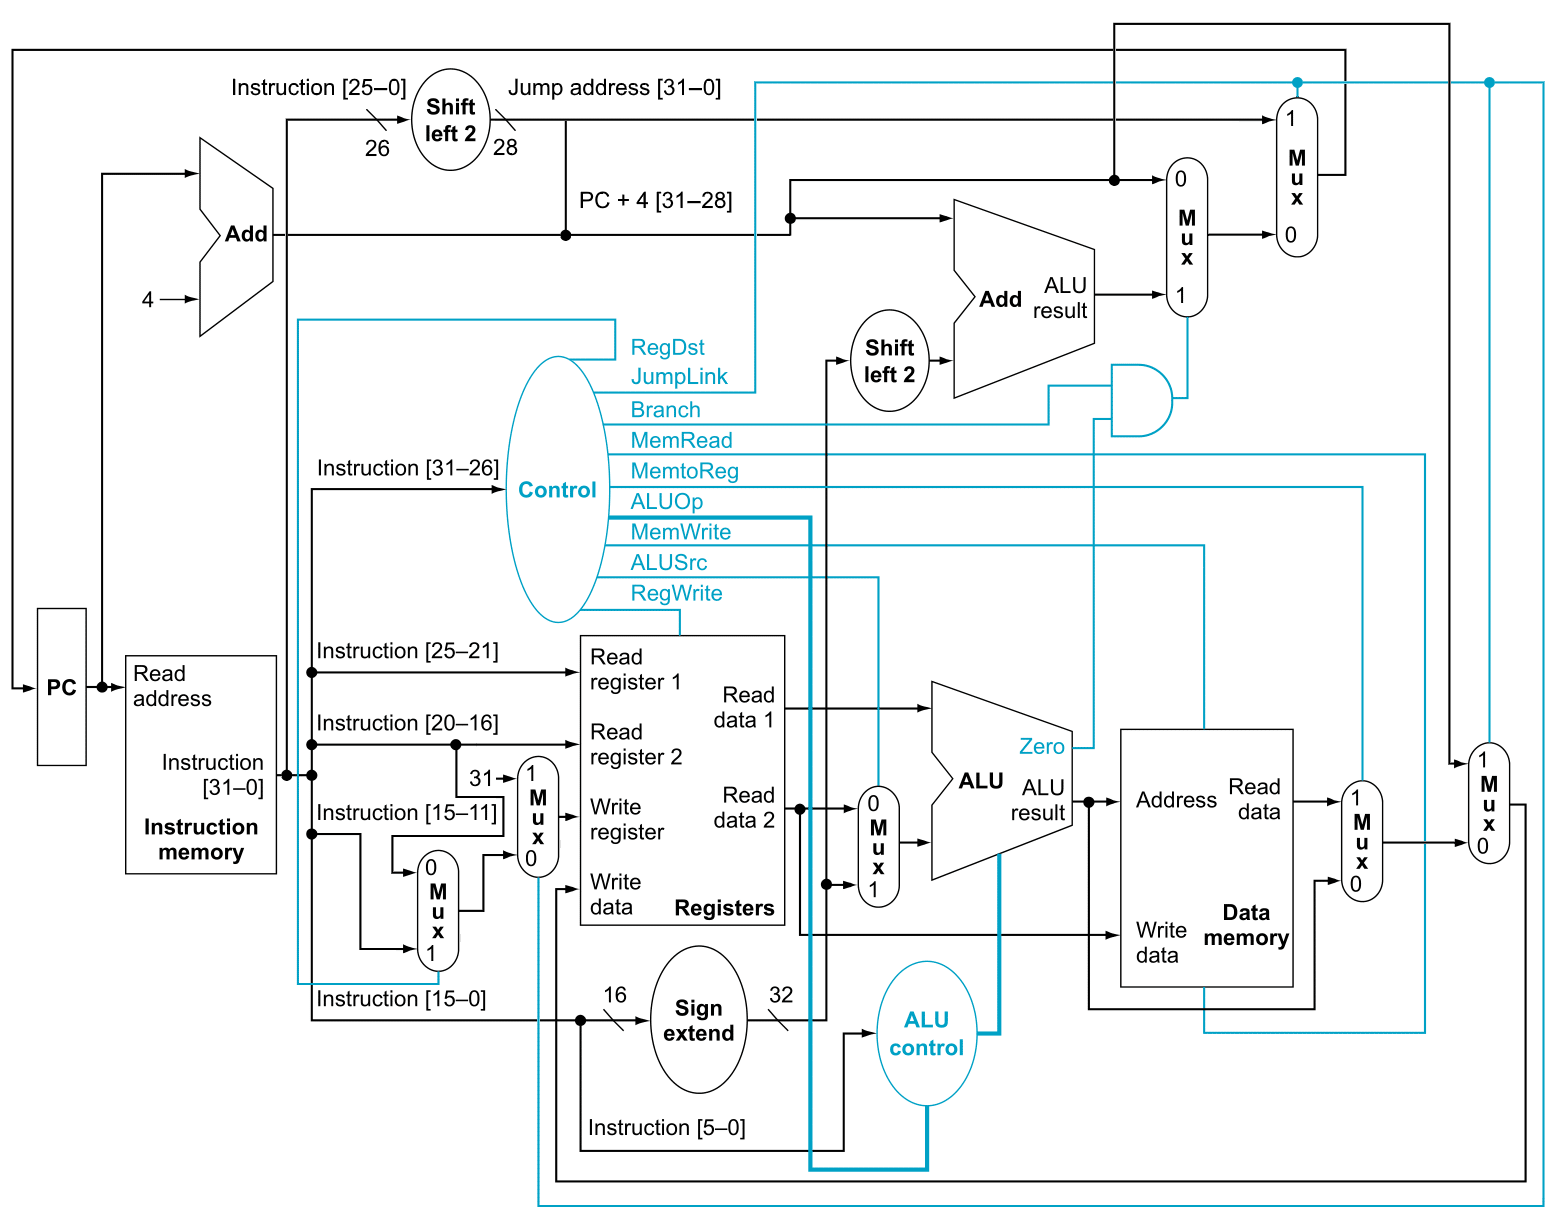
\includegraphics[width=4.4in]{problem1a.png}
    \end{center}
\end{figure}

I have added three multiplexers, one to update the program counter to the target value, one to input the next instruction as a write
value, and one to select register \(31\), which corresponds to \texttt{\$ra}. On the upper left the target value is shifted left by \(2\)
bits and the upper \(4\) bits of the program counter are concatenated on the left of the resulting value, giving a single \(32\) bit address
for the program counter to jump to. A single new control signal \texttt{JumpLink}, controls these multiplexers.

\paragraph{b)}

\texttt{JumpLink} is the new control signal required. This should be \(1\) during the \texttt{jal} instruction, and controls multiplexers that
cause the program counter to jump to the target address and saves the next instruction in register \texttt{\$ra}.

\paragraph{c)}

\begin{center}
        \begin{tabular}{c|c|c|c|c|c|c}
                Input or Output & Signal & R-Format & lw & sw & beq & jal\\
                \hline
                \multirow{6}{*}{Inputs} & Op5 & \(0\) & \(1\) & \(1\) & \(0\) & \(0\)\\
                & Op4 & \(0\) & \(0\) & \(0\) & \(0\) & \(0\)\\
                & Op3 & \(0\) & \(0\) & \(1\) & \(0\) & \(0\)\\
                & Op2 & \(0\) & \(0\) & \(0\) & \(1\) & \(0\)\\
                & Op1 & \(0\) & \(1\) & \(1\) & \(0\) & \(1\)\\
                & Op0 & \(0\) & \(1\) & \(1\) & \(0\) & \(1\)\\
                \hline
                \multirow{10}{*}{Outputs} & RegDst & \(1\) & \(0\) & x & x & x\\
                & ALUSrc & \(0\) & \(1\) & \(1\) & \(0\) & x\\
                & MemtoReg & \(0\) & \(1\) & x & x & x\\
                & RegWrite & \(1\) & \(1\) & \(0\) & \(0\) & \(1\)\\
                & MemRead & \(0\) & \(1\) & \(0\) & \(0\) & \(0\)\\
                & MemWrite & \(0\) & \(0\) & \(1\) & \(0\) & \(0\)\\
                & Branch & \(0\) & \(0\) & \(0\) & \(1\) & \(0\)\\
                & ALUOp1 & \(1\) & \(0\) & \(0\) & \(0\) & x\\
                & ALUOp2 & \(0\) & \(0\) & \(0\) & \(1\) & x\\
                & JumpLink & \(0\) & \(0\) & \(0\) & \(0\) & \(1\)
        \end{tabular}
\end{center}

\section*{Problem 2}

\section*{Problem 3}

\paragraph{a)}

\paragraph{b)}

\paragraph{c)}

\paragraph{d)}

\section*{Problem 4}

\section*{Problem 5}

\paragraph{a)}

\paragraph{b)}

\paragraph{c)}

\paragraph{d)}

\paragraph{e)}

\end{document}